\documentclass[twocolumn]{article}[10pt]
\usepackage[english]{babel} 
\usepackage[latin1]{inputenc} 
\usepackage{times} 			% Default times font style
\usepackage[T1]{fontenc} 	% Font encoding
\usepackage{amsmath} 		% Math package
\usepackage{mathtools} 		% Adds the declare paired 
							% delimeter command to make costom \abs and \norm
\usepackage{breqn}		 	% Adds dmath environment for automated brakeline
\usepackage{xfrac}			% Adds slanted fractions (sfrac)
\usepackage{cancel}			% Adds the cancel command, a slash through the symbol(s)
\usepackage{tabularx}		% Adds adjustable width on tabulars
\usepackage{cuted}			% Adds the strip command, pagewidth text in a twocolumn
							% environment. 
\usepackage{hyperref}

% Start costum \abs \norm 
\DeclarePairedDelimiter\abs{\lvert}{\rvert}%
\DeclarePairedDelimiter\norm{\lVert}{\rVert}%
% Swap the definition of \abs* and \norm*, so that \abs
% and \norm resizes the size of the brackets, and the 
% starred version does not.
\makeatletter
\let\oldabs\abs
\def\abs{\@ifstar{\oldabs}{\oldabs*}}
%
\let\oldnorm\norm
\def\norm{\@ifstar{\oldnorm}{\oldnorm*}}
\makeatother
% End costum \abs \norm 

% TODO: Put comments on this section.
\newcommand{\eq}[1]{\begin{align*}#1\end{align*}}
\newcommand{\equ}[1]{\begin{align}#1\end{align}}
\renewcommand\vec[1]{{\bf #1}}
\newcommand{\OP}[1]{{\bf\widehat{#1}}}

\title{}

\begin{document}

\begin{titlepage}
\begin{center}

\textsc{\Large Variational Monte Carlo Simulations of
Atomic Systems}\\[0.5cm]
\rule{\linewidth}{0.5mm} \\[0.4cm]
{ \huge \bfseries  Part I}\\[0.10cm]
\rule{\linewidth}{0.5mm} \\[1.5cm]
\textsc{\Large FYS4411}\\
\textsc{\Large Computational Physics II}\\[1.5cm]
\textsc{}\\[1.5cm]

% Av hvem?
\begin{minipage}{0.49\textwidth}
    \begin{center} \large
		Daniel Marelius Bj\o rnstad
    \end{center}
\end{minipage}
\begin{minipage}{0.49\textwidth}
    \begin{center} \large
        Alexander Fleischer
    \end{center}
\end{minipage}

\vfill

% Dato nederst
\large{Dato: \today}

\end{center}
\end{titlepage}

\maketitle
%\newpage

\section{Introduction}
This is part 1 of a 3 part project to evaluate the ground state properties of 
some single atoms and diatomic molecules, 
using variational Monte Carlo simulations. 

A compulsory part of doing this is using expandable programs that can handle 
systems of increasing particles and complexity. 
This poses many challenges; implementational, statistical, 
numerical and mathematical. 
The atoms studied here are Helium and Beryllium, 
and the ground state energies and one-body densities are the properties
we are interested in. The computational methods to do this is a main focus of 
part 1. 

We are interested in the ground state energies, because the
results are more easily verifiable. One aim of the project is
to see how effective our numerical methods are in computing
these quantities, and compare the methods to each other,
by applying statistical tools.

As stated, there are several challenges. Here basic mathematical,
computational, statistical models are dealt with, and applied to the second 
most simple system, Helium. 

All results displayed in this article are 
gathered from our variational Monte Carlo program. 

Github: \\ \url{https://github.com/lastis/FYS4411}

\section{Methods}
\subsection{Definitions}
The Helium atom consists of two electrons orbiting a nucleus,
where the distance between electron 1 and the nucleus,
and electron 2 and the nucleus are labeled as
$r_1 = \sqrt{x_1^2 + y_1^2 + z_1^2}$ 
and $r_2 = \sqrt{x_2^2 + y_2^2 + z_2^2}$.

The total potential energy of the system is modelled as
{\small
\eq{
    V(r_1,r_2)=-\frac{2}{r_1}-\frac{2}{r_2}+\frac{1}{r_{12}}
}}%
where the interaction between each electron and the nucleus
is given by the two first terms. 
The mutual electron-electron repulsion is given by the last.
The distance between the electrons is $r_{12}=|\vec r_1-\vec r_2|$.

The Hamiltonian of the system is thusly, 
{\small
\eq{
    \OP H = -\frac{\nabla_1 ^2}{2} -\frac{\nabla_2 ^2}{2}
    -\frac{2}{r_1}-\frac{2}{r_2}+\frac{1}{r_{12}}
}}%

%% Stating units / constants
The radii \{$r_1$, $r_2$, $r_{12}$\} are scaled, and are dimensionless.

%% The spherical nature of the wavefunction
The Laplace operator of a function $f$ in three dimensions, $\nabla^2 f$,
can be represented as
{\small
\eq{
  \bigg( \frac{\partial^2}{\partial r^2} 
    + \frac{2}{r} \frac{\partial}{\partial r} \bigg) f
    +\frac{1}{r^2 \sin\theta}\frac{\partial}{\partial \theta}
    \bigg( \sin\theta \frac{\partial}{\partial \theta}  \bigg) f
    +\frac{1}{r^2 \sin^2\theta}\frac{\partial^2}{\partial^2 \varphi} f
}}%

in spherical coordinates, and as

{\small
\eq{
	\bigg( 
	\frac{\partial}{\partial x^2} +
	\frac{\partial}{\partial y^2} +
	\frac{\partial}{\partial z^2}
	\bigg) f
}}%

in cartesian coordinates.

%% Calculating the integral using VMC and Metropolis algo.
\subsection{The Variational Principle}
The Variation Principle states that if we have a Hamiltonian
$\OP H$ and a trial wavefunction $\psi_{T}$,
an upper bound for the ground state energy is given by
equation (\ref{eq:E0var}). 

The principle is that the given integral is a
value of the energy of a given wave function and when the wave function
is variated, the according values of the energy is the output. If we then
record the lowest energy, the ground state, we also have the wave function
of the ground state. 
\begin{strip}
{
\equ{
	&E_0 \leq
	\langle H \rangle =
	\frac{\int d{\bf r_1}d{\bf r_2}\psi^{\ast}_{Ti}({\bf r_1},{\bf r_2}, 
	{\bf r_{12}})
	\OP{H}({\bf r_1},{\bf r_2}, {\bf r_{12}})
	\psi_{Ti}({\bf r_1},{\bf r_2}, {\bf r_{12}})}
	{\int d{\bf r_1}d{\bf r_2}\psi^{\ast}_{Ti}({\bf r_1},{\bf r_2}, {\bf r_{12}})
	\psi_{Ti}({\bf r_1},{\bf r_2}, {\bf r_{12}})}\label{eq:E0var}
}}%
\end{strip}


\subsection{Variational Monte Carlo (VMC)}
The integrals to be solved in the variational method,
does not scale well with traditional integral methods when 
increasing the number of particles and dimensions and using 
more complex wave functions .

Therefore, we introduce the brute-force Monte Carlo method
to solve the integrals.

\subsubsection{VMC Algorithm}

\begin{itemize}
    \item Initialization.
    \begin{itemize}    
        \item Set a fixed number of MC steps.
        \item Choose initial position $\vec R$ and variational
            parameters $\boldsymbol\alpha$.
        \item Calculate $|\psi_T(\vec R)|^2$
    \end{itemize}
    \item Set energy and variance and start the MC calculation.
    \begin{itemize}    
        \item Find the trial position $\vec R' =\vec R + \delta\times r $,
            where $r\in [0,1]$ is randomly selected.
        \item Use the Metropolis algorithm to determine if the
            move $w =\frac{P(\vec R')}{P(\vec R)}$ is accepted or rejected.
        \item Given that the move is accepted, set $\vec R = \vec R'$.
        \item Update averages.
    \end{itemize}
    \item Compute final averages.
\end{itemize}
%% End of the VMC section

\subsection{The Metropolis Algorithm}
The Metropolis algorithm samples a normalized probability distribution
by a stochastic process. In other words, it is a method for simultaing
random walks, which we can use to do brute-force Monte Carlo computations.

Define $P^{(n)}_i$ as the probability for finding the system in state $i$
at some step $n$.

\begin{itemize}
	\item Sample a possible new state $j$ with a probability $T_{i\rightarrow j}$.
	\item With probability $A_{i\rightarrow j}$, accept $j$ as a new state.
	Set it as the new sample. The move is rejected with probability $1-A_{i\rightarrow j}$.
	set $i$ as the sample again.
\end{itemize}


\subsection{Importance Sampling}
A random walker is the most efficient way to sample where the
wave function is large. To increase this we can implement importance
sampling wher the walk in space is effected by the trial wave function. 

The results are based on the Fokker-Planck equation and the Langevin 
equation. This makes the step look similar to a diffusion process
where the new position is given by,
\begin{align*}
y = x + DF(x) \delta t + \xi \sqrt{\Delta t}.
\end{align*}

$\xi $ is a gaussian random variable and $\Delta t$ is a chosen timestep.
For atomic units $D$ is $1/2$ and $\Delta t$ is a variable for the 
simulation. In our plots $\Delta t = 0.01$. 

An important part of this result is that the walker is effected by $F(x)$
which contains the trial wavefunction. This has been named the quantum 
force. 

\begin{align*}
\vec F = 2\frac{1}{\Psi_T}\nabla \Psi_T. 
\end{align*}

This also has the result of changing the random number check in the 
Metropolis algorthm from :
$q(y,x) = |\Psi_T(y)|^2/|\Psi_T(x)|^2$ to: 
\[
q(y,x) = \frac{G(x,y,\Delta t)|\Psi_T(y)|^2}{G(y,x,\Delta t)|\Psi_T(x)|^2}.
\]

Where G is the Green function given by,

\eq{
  G(y,x,\Delta t) =  \frac{1}{(4\pi D\Delta t)^{3N/2}}\\ \cdot \exp{\left(-(y-x-D\Delta t F(x))^2/4D\Delta t\right)}.
}

\subsection{Statistical Analysis}
The MC calculation are a set of computational \textit{experiments}, 
with statistical errors. In the experiments we are interested in the mean
value of the ground energies and the density distribution. The 
individual samples are not as interesting to us and we would rather like
to look in the variance of the mean value. 

	The variance of the mean value is closely connected with the correlation
in the individual samples. This can be shown mathematically, but the result
is this:
\eq{
\sigma^2(m) &= \frac{1}{n^2}\sum_{i,j=1}^{n} \mathrm{Cov}(x_i,x_j)
}

Both our random walker and walking with importance sampling gives correlated
samples. In our case, blocking is the technique of finding out have many steps
the walker has to go to be as uncorrelated as possible with it's first step.
If we then plot the variance in mean as a function of block size we 
will see that the variance reaches a plateau. 

This plateau means that increasing the sample length will no longer
change the variance in the mean significantly. This makes us able to more easily calculate 
variance in the mean because we know how short block sizes we can use. 
This is used to make the standard deviation interval around our densities. 


\subsubsection{Blocking Implementation}

\begin{itemize}
    \item Compute MC calculation, store samples in array.
    \item Loop over a set of block sizes $n_b$.
    \item For each $n_b$, calculate the mean of the block
        and store these values in a new array.
    \item Take the mean and variance of this array.
    \item Store results.
\end{itemize}

\subsection{The Trial Wavefunctions for Helium}

To conclude if the computational methods are implemented correctly,
we should check that the results are reasonable. We do this by
finding a mathematical approximation of the closed form expression.

%% The closed-form expression.
Given the trial wavefunction $\psi_T (\vec R, \boldsymbol\alpha)$, 
we define a new quantity
{\small
\eq{
  E_L = \frac{1}{\psi_T}\OP H \psi_T
}}%
where $\boldsymbol\alpha$ is a set of variational parameters.
$E_{L1}$ is called the local energy

\subsubsection{The first trial wavefunction}
We first model the variational solution with a trial function of one
variation parameter $\alpha$. It has the form
{\small
\eq{
\psi_{T1}({\bf r_1},{\bf r_2}) = 
   \exp{\left(-\alpha(r_1+r_2)\right)}
}}%

The only part of the operator $\OP H$ that affects the wavefunction
are the Laplace operators.

Since $\psi_{T1}$ is only spatially dependent on $r_1$ and $r_2$,
the Laplaces of $\psi_{T1}$ reduces to
{\small
\eq{
  \nabla_i^2 \psi_{T1} = \bigg( \frac{\partial^2}{\partial r_i^2} 
    + \frac{2}{r_i} \frac{\partial}{\partial r_i} \bigg) \psi_{T1}
    = \bigg( \alpha^2 -\alpha\frac{2}{r_i}  \bigg)\psi_{T1}
}}%
for $i = 1,\;2$, since
{\small
\eq{
  \frac{\partial}{\partial r_i} e^{-\alpha (r_1+r_2)}
    &= -\alpha e^{-\alpha (r_1+r_2)}\\
\frac{\partial^2}{\partial r_i^2} e^{-\alpha (r_1+r_2)}
    &= \alpha^2 e^{-\alpha (r_1+r_2)}
}}%
This gives us the following trial energy
{\small
\eq{
  E_{L1}&=\frac{1}{\psi_{T1}}\bigg( -\alpha^2 
  +\alpha\bigg( \frac{1}{r_1}+\frac{1}{r_1}  \bigg)
    -\frac{2}{r_1}-\frac{2}{r_2} + \frac{1}{r_{12}}
    \bigg)\psi_{T1}\\
  &=(\alpha-2)\bigg( \frac{1}{r_1}+\frac{1}{r_2} \bigg)
    +\frac{1}{r_{12}}-\alpha^2
}}%
The $2$ in the $\alpha-2$ term is the number of protons, Z.

\subsubsection{The second trial wavefunction}
To approximate the closed-form solution even better,
we assume another trial wavefunction based on $\psi_{T1}$, namely
{\small
\eq{
  \psi_{T2} ({\bf r_1},{\bf r_2}, {\bf r_{12}})
    =\exp{\left(-\alpha(r_1+r_2)\right)}
    \exp{\left(\frac{r_{12}}{2(1+\beta r_{12})}\right)}
}}%
The second part is dependent on the distance between the
electrons, and is called the correlation part,
which accounts for the effect between the electrons.

One can then in the same way as for $\psi_{T1}$ calculate
the local energy. The correlations part will give us some trouble
when we try to calculate the Laplacian. This is due to
the distance between $\vec r_1$ and $\vec r_2$, since this quantity
is dependent on the angles $\varphi$ and $\theta$.
It has the form
{\small
\eq{
	E_{L2} = E_{L1}+\frac{1}{2(1+\beta r_{12})^2}
	\bigg(\frac{\alpha(r_1+r_2)}{r_{12}}(1-
	\frac{\mathbf{r}_1^T\mathbf{r}_2}{r_1r_2})\\
	-\frac{1}{2(1+\beta r_{12})^2}-\frac{2}{r_{12}}+
	\frac{2\beta}{1+\beta r_{12}}\bigg)
}}%

\subsection{The Trial Wavefunction for Beryllium}
We can use a trial wavefunction on the same form as for
Hydrogen and Helium

{\small
\eq{
	\psi_{T}({\bf r_1},{\bf r_2}, {\bf r_3}, {\bf r_4}) &= 
 	Det\left(\phi_{1}({\bf r_1}),\phi_{2}({\bf r_2}),
	\phi_{3}({\bf r_3}),\phi_{4}({\bf r_4})\right)\\ &\cdot
   	\prod_{i<j}^{4}\exp{\left(\frac{r_{ij}}{2(1+\beta r_{ij})}\right)}
}}%

where we approximate the Slater determinant \textit{Det} as
{\small
\eq{
	\psi_{T}({\bf r_1},{\bf r_2}, {\bf r_3}, {\bf r_4})&\propto 
	\left(\phi_{1s}({\bf r_1})\phi_{2s}({\bf r_2})-\phi_{1s}({\bf r_2})
	\phi_{2s}({\bf r_1})\right)\\
	&\cdot\left(\phi_{1s}({\bf r_3})\phi_{2s}({\bf r_4})
	-\phi_{1s}({\bf r_4})\phi_{2s}({\bf r_3})\right)
}}%
where the hydrogenic wavefunctions for the two spin orbitals
are given by
{\small\eq{
\phi_{1s}({\bf r_i}) = e^{-\alpha r_i}
}} and
{\small\eq{
\phi_{2s}({\bf r_i}) = \left(1-\alpha r_i/2\right)e^{-\alpha r_i/2}
}}

\subsection{Onebody Density and Charge Density}
The one-body density is computed from the form 
{\small
\eq{
	\rho(\vec R) = |\psi(\vec R)|^2
}}%

This is implemented as NOTE: ... in our program. 

\subsection{Implementation}
The methods described above are implemented in an object oriented C++ program
which is simple to use, and does not have any dependencies. 

Most of the code is contained in the class VMCSolver.cpp and VMCSolver.h. 
These were created to contain the full system and parameters for a single run. 

To start a simulation one must instantiate the solver and 
initialize the system, either by file and/or manually. After this
the integration can be run and all data will be contained in the solver object.
The last step is to collect data from the solver. 

All plot data are generated by individual programs using the mentioned solver. 
Plots are generated using python. 

\section{Results}
\subsection{Helium: Estimating $\alpha$ and $\beta$}
These parameters decide the minimal ground energy for the system, and both
should be adjusted simultaneously to reach the most optimal value of the
energy. First we sample the parameterspace of the first trial wave function. 
This function had a minimum of 1.66. This was the first value of $\alpha$ that was used in sampling the 
parameterspace with beta in the second trial wavefunction. 
This can  be seen in Figure \ref{fig:1} with mean error. 
Using the computed $\beta$-value we again
sampled the energy as a function of $\alpha$, which we concluded was 
the same as before. $\alpha$ is plotted in Figure \ref{fig:2}

\begin{figure}[h!]
	\centering
	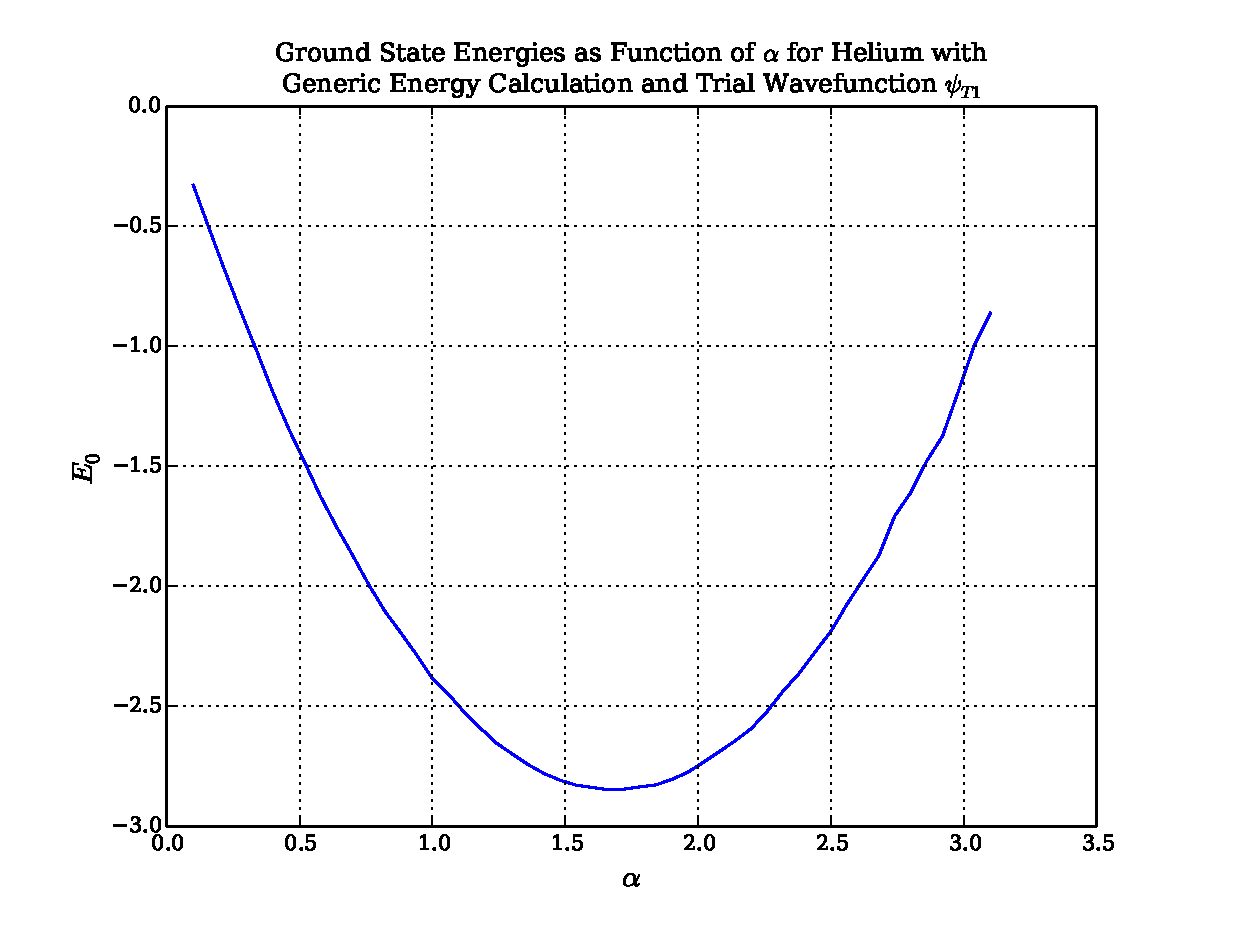
\includegraphics[width=80mm]{../res/heliumWave1Alpha/heliumWave1Alpha_alpha.eps}
	\caption{}\label{fig:2}
\end{figure}

\begin{figure}[h!]
	\centering
	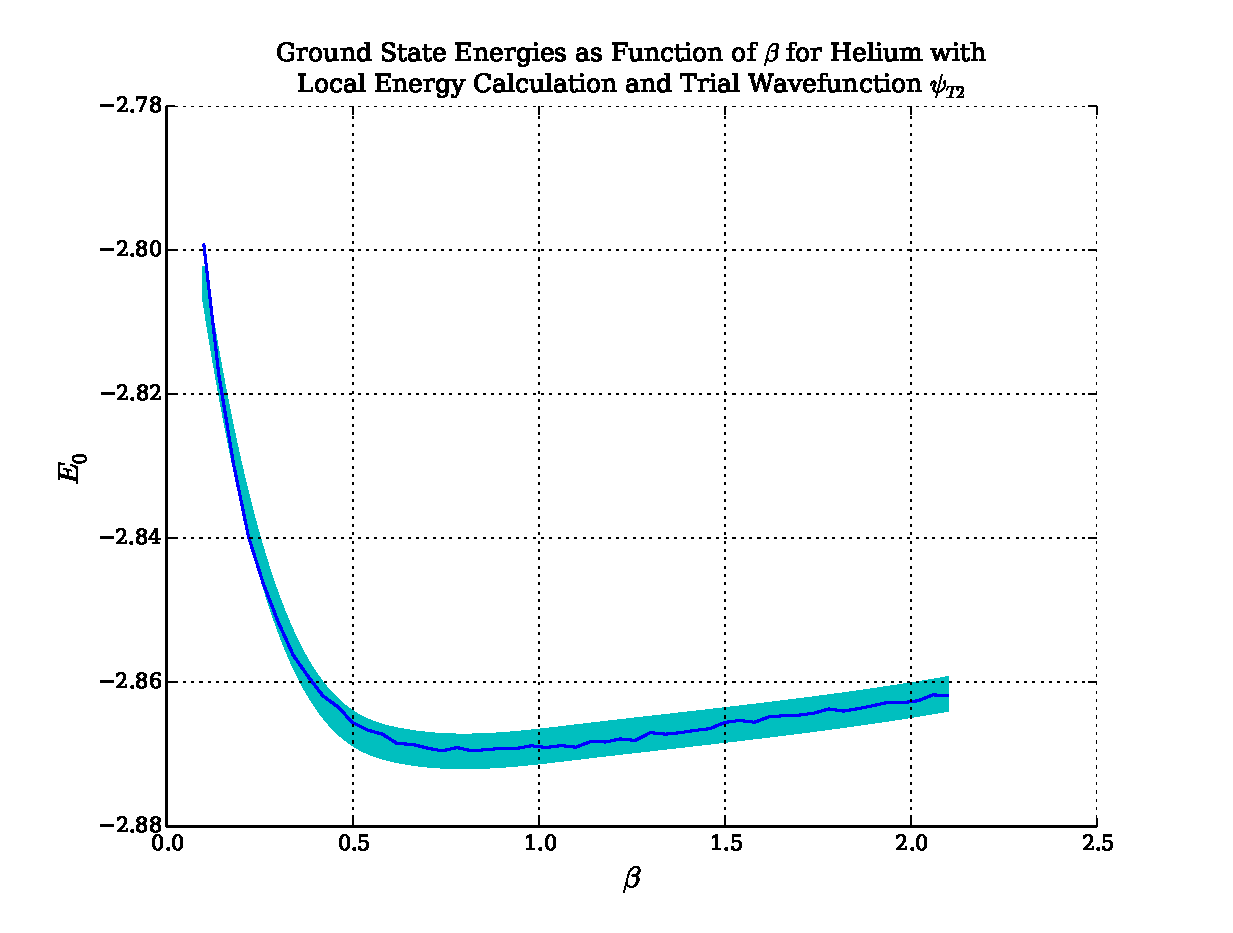
\includegraphics[width=80mm]{../res/heliumWave2Beta/heliumWave2Beta.eps}
	\caption{}\label{fig:1}
\end{figure}

\subsection{Helium: $\psi_{T1}$ and $\psi_{T2}$ }
Firstly we want to compare the first and second trial wavefunctions for Helium. 
The difference between these two are that there are no correlation term
in the first wavefunction. This makes computations much faster, but we
would expect that our results are farther away from the experimental 
value of the ground state. This is done using a numerical approximation 
of the local energy of the particles. The mean value of 
$\psi_{T1} = -2.84264$ and $\psi_{T2} = -2.87105$. The experimental value of
the ground state is about $-2.903$, thus we conclude that the second wavefunction is a better approximation.

\subsection{Helium: Closed Form Local Energy}
The local energy has a closed form solution for Helium, this has 
been implemented in Figure \ref{fig:3}. The closed-form solution should
give use a lower standard deviation than the numerical approximation
of the local energy because it is a closer approximation. 

\subsection{Helium: Importance Sampling}
Now we would like to see how the program does with importance sampling instead 
of static steplength. Importance sampling should also lower the standard 
deviation because it makes the walker sample the wavefunction in a
better way. The downside of importance sampling is that it takes about
twice as long time as the random walker. This is also shown in Figure \ref{fig:3}. 

\begin{figure}[h!]
	\centering
	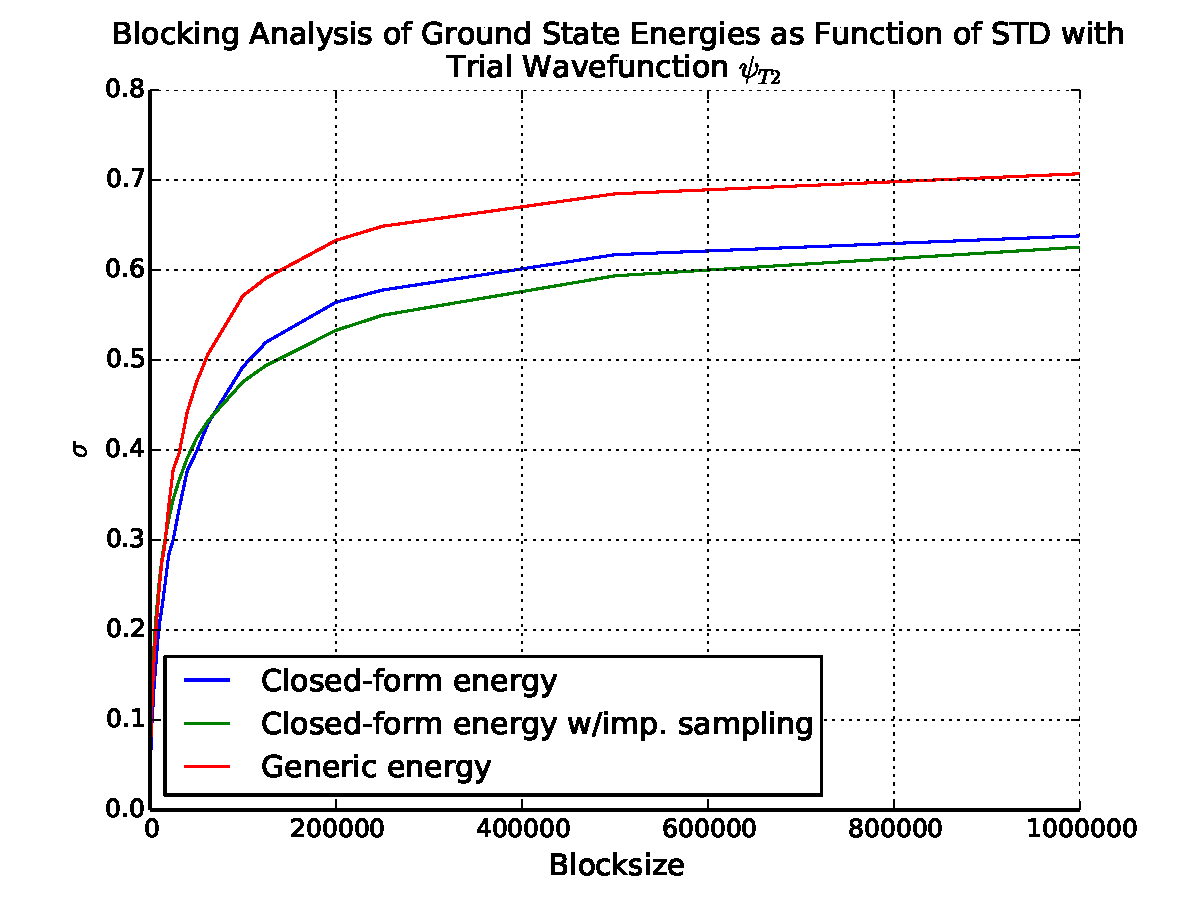
\includegraphics[width=80mm]{../res/heliumWave2ClosedImportanceGeneric/heliumWave2BlockingClosedImpGen.pdf}
	\caption{}\label{fig:3}
\end{figure}

\subsection{Helium: Evaluating Ground State and Density}
With our optimal parameters, we calculated the ground state and the density
function of Helium, Figure \ref{fig:4}. The standard deviation has been added as
a error bar along the curve.

Here we can see how the correlation factor effects the density. When
the Jastrow factor is added the electrons are repelled a bit farther 
away from the nucleus and the mean radius between the electrons increases
slightly. The mean distance increased from $1.316$ to $1.414$. 
\begin{figure}[h!]
	\centering
	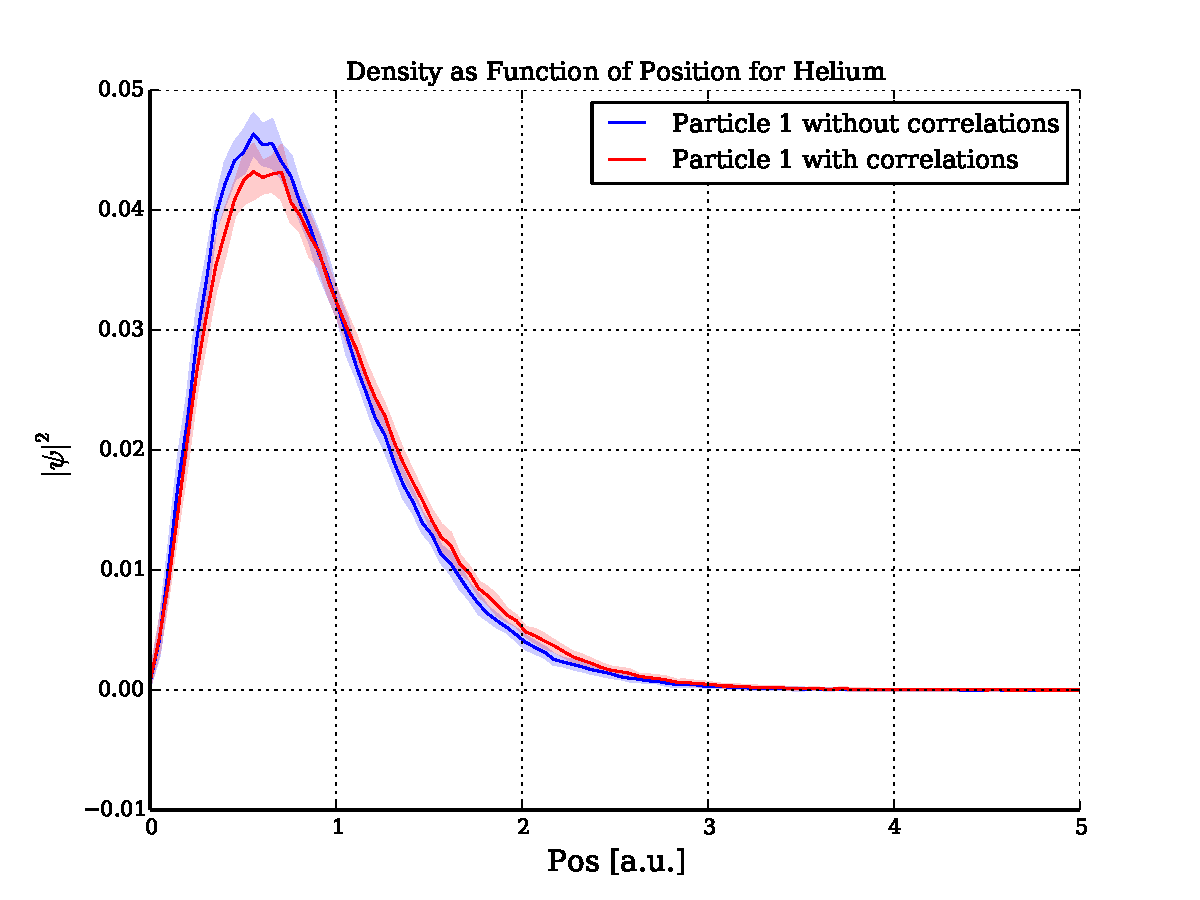
\includegraphics[width=80mm]{../res/heliumWave1Wave2Density/heliumWave1Wave2DensityPos1.pdf}
	\caption{}\label{fig:4}
\end{figure}

\subsection{Beryllium: Estimating $\alpha$ and $\beta$}
In Figure \ref{fig:5} a wide range of the parameter space has been sampled. As can be seen this area have an energy mean that are quite similar. Because of this
the parameters have been chosen to be $\alpha =  3.75$ and $\beta = 0.8$. 
\begin{figure}[h!]
	\centering
	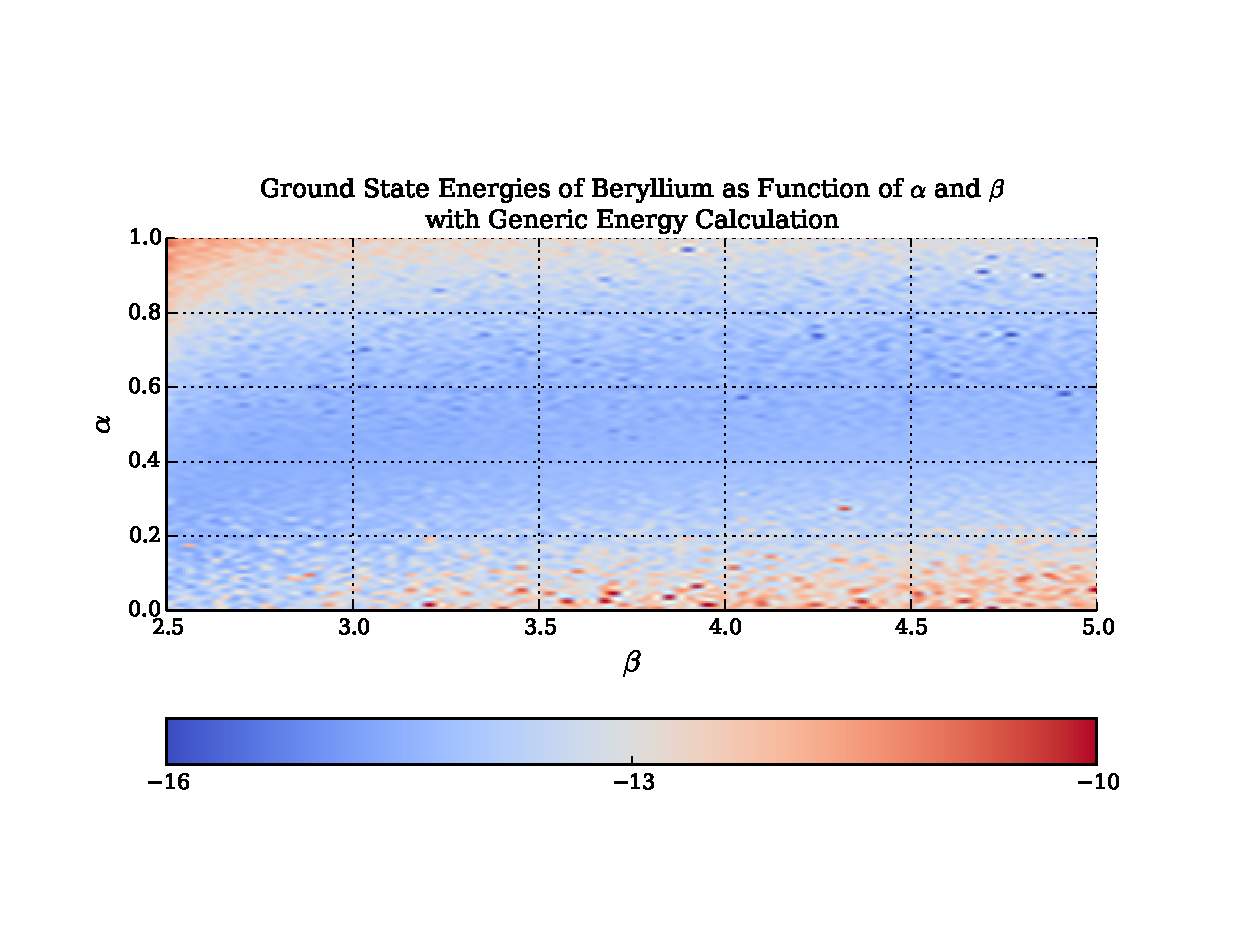
\includegraphics[width=80mm]{../res/berylliumAlphaBeta/berylliumAlphaBeta.eps}
	\caption{}\label{fig:5}
\end{figure}

\subsection{Beryllium: Comparing $\psi_{T1}$ and $\psi_{T2}$}
In Figure \ref{fig:6} we see the difference the Jastrow factor makes for Beryllium. 
We also notice the two clear peaks in the distribution. These are
the electron orbitals for 1s and 2s. Again this
correlation makes the electrons repel each other and pushes the distributions
farther apart. The mean distance increased from $1.669$ to $1.804$. 
The mean energy were $-19.9325$ and $-14.340$ respectively. A walue around
$-14$ is the experimental value of Beryllium and the value without the 
Jastrow factor is supposed to be $-20$. 
\begin{figure}[h!]
	\centering
	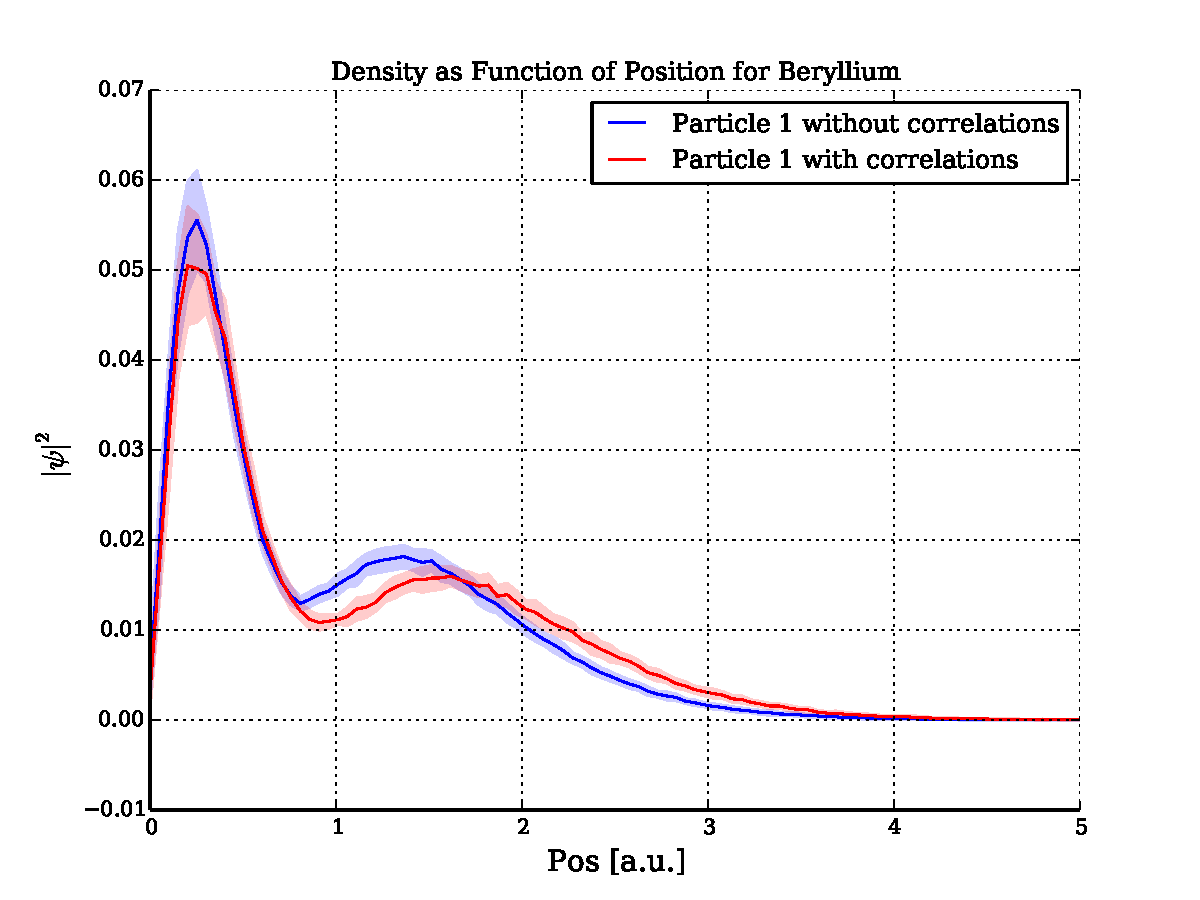
\includegraphics[width=80mm]{../res/berylliumWave1Wave2Density/berylliumWave1Wave2DensityPos1.pdf}
	\caption{}\label{fig:6}
\end{figure}




\section{Discussion}
\subsection{Parameter Space}
After estimating the parameters $\alpha$ and $\beta$ for 
Helium, we didn't adjust them in the late comparative trials. The reason
for this was that small changes in the parameters did not effect
our results considerably because the mean energies as well as the variance of the mean energies are similar. Our results was always close to 
$=-2.89$. The same conclusion was made for Beryllium, which
showed even harder to locate exact values of the paramters.  

The standard deviation of the mean was not considered when estimating the values 
of $\alpha$ and $\beta$. Performing blocking with our program would require full 
sampling of every step which stores about 10 mb for every value of $\alpha$ and $\beta$. 
\subsection{Testing of the Solver}
To varify that the solver works as intended, several unit tests
using UnitTest++ were created. The most important tests 
are those that estimate the one-body hamiltonian. this has
an analytical solution for both Helium and Beryllium, which is $-4$
and $-20$ respectively. 

The solutions for Hydrogen are also easy to calculate, and was estimated
to be $-0.5$ correctly.

\section{References}

\noindent Monte Carlo: Morten Hjorth-Jensen, Computational Physics, Lecture Notes Fall 2014, p. 345 (2014)\\

\noindent Importance Sampling: Morten Hjorth-Jensen, Computational Physics, Lecture Notes Fall 2014, p. 370 (2014)\\

\noindent Metropolis Algorithm: Morten Hjorth-Jensen, Computational Physics, Lecture Notes Fall 2014, p. 401 (2014)\\

\noindent Metropolis Algorithm: NICHOLAS
METROPOLIS,
ARIANNA
W.
ROSENBLUTH,
MARSHALL
N.
ROSENBLUTH,
AND
AUGUSTA
H.
TELLER,
Los
Alamos
Scientific
Laboratory,
Los
Alamos,
New
Mexico and EDWARD
TELLER,
*
Department
of
Physics,
University
of
Chicago, Chicago,
Illinois, The Journal of Chemical Physics \textbf{21}, p. 1087 (1953)\\

\noindent Blocking: H. Flyvbjerg and H. G. Petersen: Averages of correlated data, The Journal of Chemical Physics \textbf{91}, p. 461 (1989)
\end{document}
